\chapter{Einleitung}
Durch die voranschreitende technische Entwicklung in Industrie, Gewerbe und Landwirtschaft verändert und belastet der Mensch zunehmend die Umwelt.
Umweltbelastungen können viele Ursachen haben, möglicherweise sind bessere Lösungen technisch
nicht umsetzbar oder wirtschaftlich unattraktiv.
Die Umweltbelastung entsteht auf verschieden Ebenen, die sich in ihrer Gegebenheit unterscheiden.
Es gibt energetische Belastungen, wie Strahlen, Lärm und Erschütterungen.
Belastungen durch feste Stoffe wie Abfälle welche durch Bau und Abbruch entstehen,
Abfälle aus Produktionen und
Abfälle aus der Gewinnung von Bodenschätzen.
Auch flüssige Stoffe belasten die Umwelt.
Sie entstehen durch Chemie Fabriken,
Reste von Medikamenten die durch den Urin in das Abwasser gelangen oder
durch Umweltkatastrophen bei der sich das Wasser mit andren Stoffen vermischt.
Ein Beispiel hierfür könnte ein Erbebben sein,
welches ein Atomkraftwerk beschädigt und radioaktives Wasser ausläuft.
Die größte Belastung für die Umwelt ist aber die gasförmige Verschmutzung, in From von Luftschadstoffen und Feinstaub.
Durch unsachgemäße Wiederverwertung können Luftverschmutzungen entstehen,
wie zum Beispiel die Verbrennung von
Stromkabeln um das Kupfer aus der Isolierung zu trennen.
Die Luftverschmutzung ist ebenso verantwortlich für Krankheiten und vorzeitigen Tod von Menschen.
Feinstaub kann in den Körper eindringen und schwerwiegende Krankheiten auslösen.
Luftverschmutzung entsteht bei Tierhaltung sowie durch den Einsatz von Pestiziden.
Eine Ursache sind Abgase die bei der Verbrennung von fossilen Kraftstoffen erzeugt werden.

\section{Ausgangssituation}
Die Folge von globaler Erwärmung sowie die Veränderung des Klimas sind allgegenwärtig und betreffen den gesamten Globus.
Regionale Veränderungen von Wetter werden fallen immer häufiger extremer aus.
Starke unregelmäßige Wetterereignisse führen können zu materiellen Schäden an Gebäuden und Infrastrukturen vor allem aber nennenswerte Ertragsverluste der Landwirtschaft.
Die globale Erderwärmung steigt kontinuierlich an.
% Benötigt werden Maßnahmen, die sich an unsere Umwelt anpassen kann, 
% und weitreichende Anstrengungen zur Reduzierung von Umweltbelastungen durch menschliches Handeln. 
Stark betroffen sind Entwicklungs- und Schwellenländer, die mit Überschwemmungen oder Hitzewellen zu kämpfen müssen.

% Die Resultate der Umweltkatastrophen sind verehrend.

Luftschadstoffe haben massive negative Auswirkungen auf unsere Gesundheit.
Viele Menschen sind Feinstaubwerten ausgesetzt, die sie als gesundheitsschädlich für den Menschen eingestuft werden können.
Die Reduktion von Feinstaub ist daher ein wichtiger Teil der Ausgangssituation, die für eine Begrenzung der Erderwärmung unternommen werden müssen.

Deswegen werden in dieser Fallstudie verschiedene Einsparpotenziale für Umweltbelastungen durch autonome Kraftfahrzeuge untersucht.


\section{Ziel der Arbeit}
Das Ziel dieser Arbeit ist die folgende Forschungsfrage nach dem aktuellen Stand der Technik zu beantworten:
\textit{Welche Auswirkungen haben Kraftfahrzeuge auf die Umwelt und wie kann autonomes Fahren die negativen Auswirkungen reduzieren?}
Mithilfe von frei zugänglicher Literatur soll diese Frage bearbeitet werden.
Folgende Hypothese wird untersucht:
\textit{Je mehr Fahrzeuge autonom fahren, desto geringer fällt die Feinstaubbelastung durch Kraftfahrzeuge aus}

\section{Aufbau der Arbeit}



% Anhand der technologischen Entwicklung, erster Testfelder, sowie Prototypen Industrie stellt  die Frage,
% welche Umwelteffekte beim autonomen Fahren auftreten werden.
% Dies hängt mitunter mit neuen Antriebsformen (z. B. Elektroantrieb) und Betriebsmodellen (z. B. geteilte
% Fahrzeuge) zusammen.

% Je nach der Entwicklung in den einzelnen Bereichen werden auch sich unterschiedliche Kraftfahrzeuge bei einer Einführung des autonomen Fahrens
% durchsetzten.
% Als Umwelteffekte des Autonomen Fahrens bezeichnet man die Einflüsse die sich durch autonomen Fahren ändern, hierbei kann es zur Verringern oder Anstieg von Schadstoffausstößen kommen, oder eine
% Veränderung in der Infrastruktur, da Parkplätze oder Seitenstreifen nicht mehr in gleicher Zahl benötigt werden oder der Ausbau von Straßen da das Verkehrsaufkommen zugenommen hat.
% Der Umstieg auf autonomes Fahren erfolgt nicht in einem Schritt,
% sondern schrittweise oder je nach Fahrzeugs
% nur für einzelne Anwendungsfälle (siehe Anlage I, Stufen der Automatisierung, autonomes
% Fahren bei Level 5). Im Öffentlichen Verkehr (ÖV) könnten sich Veränderungseffekte schneller einstellen.

% Denn durch den Verkehr verursachten Schadstoffe sind eine wesentliche Ursache für den schnell voranschreitenden Klimawandel.











\subsection{Klimaschutzziele}
Wer bestimmt Klimaschutzziele?
Welche Klimaschutzziele gibt es?
Welche Klimaschutzziele sollen erreicht werden?



\newpage



































% \section{LKW}
% In den Marktstudien wird darauf verwiesen, dass sich die Wirkungen vor
% allem aus Einsparungen bei den Personalkosten und bei den Kraftstoffkosten
% zusammensetzen. PwC sieht durch Platooning ein Einspareffekt bei den
% Kraftstoffkosten von rund 7Prozent. Roland Berger beziffert den Einspareffekt in
% Höhe von 8 Prozent für das führende Fahrzeug und in Höhe von 14Prozent für die
% folgenden Fahrzeuge bei einer Geschwindigkeit von 85 km/h.16 Das
% International Transport Forum beziffert die Kraftstoffkosteneinsparungen
% (infolge verbesserten Brems- und Beschleunigungsverhaltens) bei
% automatisiertem „eco-driving“ (keine Platoons) in Höhe von 4-10Prozent, bei
% teilweise manuell gesteuerten Platoons in Höhe von 6-10Prozent und bei
% vollautomatisierten Platoons bei über 10Prozent



% Klima-/Umwelteffekte



% \section{Infrastrukturen für Autonomes Fahren}
% Die Entwicklung der Zukunftstechnologien und des Markthochlaufs von autonomen Fahrzeugen (Level 4, 5) erfordert neben der Weiterentwicklung von Fahrzeugtechnologien für Autonomes Fahren (Level 5) auch materielle (5G, Datenstandards,)
% immaterielle (z.B. Software/AI-Kompetenzen) und institutionelle Infrastrukturen
% (rechtlich-regulativer Rahmen) als Erfolgsvoraussetzungen
% \subsection{Materielle Infrastrukturen: Datenübertragung (5G), Datenstandards}
% Als wesentliche technische Voraussetzungen für autonomes Fahren gelten Sensortechnologien, Software-Algorithmen und hochauflösende Karten. Für letzteres
% haben die deutschen Hersteller durch den Kauf des Kartenanbieters Here bereits
% die Voraussetzungen geschaffen. Gleichzeitig ist jedoch auch die Datenkommunikation zwischen Fahrzeug und Straßeninfrastruktur (Vehicle-to-Infrastructure) sowie der Fahrzeuge untereinander (Vehicle-to-Vehicle) und zu großen Rechenzentren (z.B. der Hersteller) fundamental. Das autonom fahrende Auto muss zu anderen
% Fahrzeugen eine Verbindung herstellen und ihnen Dinge mitteilen können, die es
% selbst gelernt hat.102 Reaktionsschnelle Mobilfunknetze (5G) sowie Datenstandards
% für einen breitbandigen und sicheren Datenaustausch sind hierfür essentiell.103
% So produzieren autonome Fahrzeuge exponentiell ansteigende Mengen an Daten
% durch ihre Sensorik wie Laser- (Lidar), Radarsensoren und Kameras, die sich auf
% 4.000 Gigabyte täglich summieren können. In cloudbasierten Datenpools werden
% diese Datenströme der autonom fahrenden Autos in Echtzeit in Datensätze verwandelt und an das Auto zurückübermittelt, damit es seine gesamte Umgebung
% erkennt. Dabei spielen Anwendungen der Künstlichen Intelligenz (KI) und des
% maschinellen Lernens eine entscheidende Rolle.104
% Gleichzeitig stellen 5G-Funkkomponenten für autonome Fahrzeuge eine
% zusätzliche Schutzebene bereit, indem diese mit Fahrzeugen im näheren Umfeld
% und der Infrastruktur am Straßenrand zuverlässig und schnell kommunizieren,
% z.B. wenn die Sensoren keine Sichtverbindung haben oder nachteilige Wetterbedingungen herrschen.105 Darüber hinaus könnten 5G-Netze mit geringen Latenzzeiten auch die Fernsteuerung autonomer Fahrzeuge ermöglichen. Flottenbetreiber
% von autonomen Fahrdiensten könnten dann in Fällen, in denen das Fahrzeug überfordert ist, mittels Fernsteuerung eingreifen. Allerdings dürften künftig sicherheitskritische Funktionen von autonomen Fahrzeugen nicht auf Mobilfunkverbindungen angewiesen sein. So gibt etwa die Google-Tochter Waymo an, dass ihre
% Fahrzeuge auch ohne eine ständige Verbindung sicher funktionieren würden.
% Prinzipiell sieht auch das Bundesverkehrsministerium 5G in der Mobilität als
% zwingende Infrastrukturvoraussetzung,106 wobei das geplante 5G-Netz für zahlreiche Zukunftstechnologien ein Engpassfaktor darstellt, darunter das Internet
% of Things (IoT).107 Heutige Festnetz-, Mobilfunk- und Satellitennetze sind nicht
% für Datenaufkommen, Reaktionsgeschwindigkeiten und die Versorgungssicherheit des Autonomen Fahrens ausgelegt. Automobilhersteller wie VW, Daimler und
% BMW haben sich bereits 2016 in der 5G Automotive Association (5GAA) zusammengeschlossen, um die notwendige Standardisierung für vernetzte und autonome
% Fahrzeuge voranzutreiben. Allerdings gibt es selbst zwischen den in der 5GAA versammelten Herstellern noch Wettstreite um technische Konzepte und Kommunikationsstandards.108 Prognosen gehen daher davon aus, dass die Hochlaufphase für
% 5G sich erst ab 2023 stark intensiviert und dann bis 2028 auch alle regulatorischen
% Fragen abgeschlossen sein werden.109
% Insgesamt sind 5G-Netze für Autonomes Fahren und das vernetzte Fahrzeug
% von großer Bedeutung, da dadurch erst sichere kommerzielle Anwendungen von
% vernetzten und autonomen Fahrzeugen möglich sind. Entsprechend muss deren
% Aufbau beschleunigt und weiter intensiviert werden. Die Investitionen in den
% 5G-Aufbau werden in einer 2016 veröffentlichten Studie für die EU-Kommission
% bis 2025 auf rund 56 Mrd. Euro veranschlagt. Dieselbe Studie prognostiziert
% im Gegenzug bis zu 113 Mrd. Euro zusätzliche Umsätze durch 5G in vier Sektoren, darunter auch Automotive, sowie die Schaffung von 2,3 Mio. Arbeitsplätzen
% europaweit.11



% \chapter{Mobilitätsdienstleistungen und deren besondere Infrastrukturvoraussetzunge}
% \section{Konzept, Klima-/Umweltrelevanz, Markttrends}
% Mobilitätsdienstleistungen sind ein zentrales Zukunftsfeld für Automobilhersteller,
% Digitalplayer wie Google, Start-ups wie Uber sowie von Städten und Kommunen
% gleichermaßen. Die Vision eines «Mobility as a Service» (MaaS) beschreibt die Vision
% einer bruchlosen, hoch vernetzten Reise- bzw. Mobilitätskette über verschiedene
% Verkehrsträger hinweg: von der intermodalen Routenplanung über die Buchung on
% Demand und der Bezahlung bis hin zur Abwicklung der Fahrten.123 Darüber hinaus
% können noch weitere Services wie Parkplatzdienste, Charging-Dienste oder Entertainment-Dienste hinzugezählt werden (vgl. für eine Übersicht Abb. 7).
% Aus Kundensicht erweitern sich durch die neuen Mobilitätsangebote wie
% Car-Sharing, Bike- und Ride-Sharing die Mobilitätsangebotsoptionen. War bis vor
% kurzem ein eher monomodales Verkehrsverhalten dominant, das alle Fahrten entweder mit dem privaten Auto oder mit dem ÖPNV vorsah, entwickelt sich mittels
% internetfähiger Smartphones ein intermodales oder gar multimodales Mobilitätsmuster: D.h. Kunden können ihren Mobilitätsbedarf individuell und schnell per
% Fingertipp mit einer breiten Vielfalt von Mobilitätsangeboten befriedigen und dabei
% nach ihren Präferenzen die günstigste, schnellste oder komfortabelste Kombination von Verkehrsmitteln auswählen. Durch multimodale Apps wie Moovel, Qixxit,
% Ubigo oder Whim kann die Reisekette mit dem Smartphone künftig in Echtzeit
% einfach und sicher geplant, gebucht und teilweise bereits bezahlt werden. Das
% Fernziel ist Interoperabilität, also die bruchlose Übersicht, Verfügbarkeit und Buchbarkeit als kundenindividuell optimierter Mix aus allen Mobilitätsangeboten –
% ÖPNV, Taxi, Car-Sharing, Ride-Hailing und Ride-Sharing, Leihwagen oder BikeSharing etc. – für die urbane Mobilität.124
% Mobilitätsdienstleistungen bzw. MaaS begründen gleichzeitig neue Geschäftsmodelle auf Basis der Mobilitätseffizienz-, der Mobilitätszeit- und der Mobilitätssystem-Revolution. Für Automobilhersteller ergibt sich durch Mobilitätsdienstleistungen in Kombination mit dem Autonomen Fahren die Chance von neue
% Geschäftsfeldern als Ersatz für die sich perspektivisch auflösenden bisherigen
% kommerziellen Pfeiler, die wesentlich auf den Autokauf bzw. Autobesitz und
% Freude am manuellen Autofahren angelegt waren.125 Gleichsam erweitert sich
% jedoch auch das Wettbewerbsumfeld durch Digitalplayer wie Apple, Google
% oder Alibaba und Baidu, die ihre Ökosysteme aus Kommunikations- und Entertainment-Services um Mobilitätsdienste erweitern wollen. Außerdem drängen
% Start-ups wie Uber, Lyft, BlablaCar und andere mit innovativen Services einer
% digitalen Mobility-on-Demand auf den Plan.
% Hinzu kommt, dass künftig mit den oben skizzierten Trends von Elektromobilität und autonomen Fahrzeugen bzw. Robo-Taxis weitere innovative und kostengünstige Mobilitätsangebote marktreif sein werden. Diese werden nicht nur
% das Spektrum von Mobilitätsdienstleistungen erweitern. Sie führen auch zu einem
% Verschmelzen von öffentlichem und privatem Verkehr, weil das autonome Fahrzeug prinzipiell sowohl privat genutzt als auch als Taxi, Car-Sharing-Fahrzeug
% oder Rufbus eingesetzt werden kann.126 Dabei stellt sich auch die Frage, ob durch
% die sich entwickelnden autonomen Fahrdienste der ÖPNV kannibalisiert wird
% oder ob diese einen positiven Beitrag zur Minderung des Autoverkehrs bzw. der
% Klimabelastung des Verkehrs leisten können.

% \subsection{Umwelt-/Klimarelevanz}
% Die lokale bzw. regionale Ebene wird eine wichtige Rolle bei der Ausgestaltung
% der Mobilitätsdienstleistungen der Zukunft spielen und damit auch bei der Frage,
% ob die neuen Angebote einen positiven Beitrag für den Klimaschutz im Verkehrsbereich erbringen können.127 Städte und Kommunen sind nicht nur mit
% der Verkehrsplanung, den baulichen Infrastrukturen von Straßen und Parkplätzen und dem Betrieb des öffentlichen Personennahverkehrs betraut. Sie können
% auch über die Ausgestaltung von integrierten Mobilitätsdienstleistungen mitentscheiden. Dabei ist der verkehrsplanerische Handlungsdruck in urbanen Gebieten
% aufgrund zunehmender Flächenknappheit bei einem gleichzeitig wachsenden
% Verkehr und Mobilitätsbedürfnis der Menschen hoch.
% Eine zentrale Bedeutung kommt den Robo-Taxis bzw. autonomen Fahrangeboten zu, bei denen noch nicht klar ist, ob sie in der Gesamtbilanz positive
% oder negative Umwelt- und Klimaeffekte haben werden (vgl. Kapitel 4). So werden zu Beginn der 2020er Jahre erste autonom fahrende Shuttles auf deutschen Straßen unterwegs sein und sich wahrscheinlich dynamisch entwickeln.
% Studien rechnen bis zum Jahr 2030 damit, dass bereits 37 Prozent des PKWVerkehrsaufkommens autonom bzw. in geteilten Systemen (Car Pooling, RideSharing) absolviert werden könnten.128 Es ist damit zu rechnen, dass die
% Automatisierung des Fahrens erhebliche Auswirkungen auf das Preisgefüge und
% damit die Nutzung der Mobilitätsservices besitzen wird.129 Robo-Taxen könnten
% Berechnungen zufolge bis zu 60 Prozent günstiger betrieben werden als konventionelle.130 In den Möglichkeiten der Kombination von autonomen Taxen und
% Sharing-Konzepten liegt dabei enormes Potenzial für die Reduzierung des Fahrtaufkommens. Unter heute geltenden Regulierungsvorschriften (u.a. Personenbeförderungsgesetz, gesetzliche Regelungen für autonomes Fahren) ist allerdings
% unklar, ob und wie dieses Potenzial gehoben werden kann.131 Es wird hierbei
% wesentlich auch auf eine umweltgerechte Flankierung und Ausrichtung der politischen Regulation bzw. Anreizstrukturen ankommen, insbesondere auch auf
% Ebene der Kommunen. Dabei müssen autonome Fahrangebote in ein multimodales Verkehrssystem integriert werden.
\chapter{Umweltbelastung}
Durch die voranschreitende technische Entwicklung in Industrie, Gewerbe und Landwirtschaft verändert und belastet der Mensch zunehmend die Umwelt.
Umweltbelastungen können viele Ursachen haben, möglicherweise sind bessere Lösungen nicht umsetzbar oder wirtschaftlich nicht attraktiv.
Die Umweltbelastung entsteht auf verschieden Ebenen, die sich in ihrer Gegebenheit unterscheiden.
Es gibt energetischen Belastungen, wie Strahlen, Lärm und Erschütterungen.
Es gibt Umweltbelastungen durch feste Stoffe wie Abfälle die durch Bau und Abbruch entstehen, Abfälle aus Produktionen und Abfälle aus der Gewinnung von Bodenschätzen.
Auch flüssige Stoffe belasten die Umwelt. Sie entstehen durch Chemie Fabriken, Reste von Medikamenten die durch den Urin in das Abwasser gelangen oder durch Umweltkatastrophen bei der sich das Wasser mit andren Stoffen vermischt.
Ein Beispiel hierfür könnte ein Erbebben sein, welches ein Atomkraftwerk beschädigt und radioaktives Wasser ausläuft.
Die größte Umweltbelastung für die Umwelt ist aber die gasförmige Verschmutzung, welche die Luft verschmutzt.
Die Gasformringe Verschmutzung welche die Luft verunreinigt ist die eine von den größten Belastungen für die Umwelt.
Durch unsachgemäße Wiederverwertung können Luftverschmutzungen entstehen, wie zum Beispiel die Verbrennung von
Stromkabeln um das Kupfer aus der Isolierung zu trennen.
Die Luftverschmutzung ist ebenso verantwortlich für Krankheiten und vorzeitigen Tod von Menschen.
Feinstaub kann in den Körper eindringen und schwerwiegende Krankheiten auslösen.
Luftverschmutzung entsteht bei Tierhaltung sowie durch den Einsatz von Pestiziden.

Die Hauptursache sind Abgase die bei der Verbrennung von fossilen Kraftstoffen entstehen.
Ein großer Träger bei der Verbrennung von fossilen Kraftstoffen sind Kraftfahrzeuge.

\section{Kraftfahrzeuge}
Das deutsche Straßenverkehrsgesetz beschreibt Kraftfahrzeuge als Landfahrzeuge, die durch Maschinenkraft bewegt werden, aber nicht an Bahngleise gebunden sind.
\footnote{Straßenverkehrsgesetz, § 1 Abs. 2}



Da Kraftfahrzeuge Landfahrzeuge sind gehören Flugzeuge, Schiffe oder Boote nicht zu der Kategorie, obwohl sie durch Maschinenkraft bewegt werden.
Auch Züge oder Trambahnen gehören nicht in in die Kategorien, da sie an Bahngleise gebunden sind.

\subsection{Teilsysteme von Kraftfahrzeugen}
Moderne Kraftfahrzeuge werden aus folgenden Teilsysteme gebildet:
\begin{itemize}
	\item Antriebseinheit
	\item Energieübertragungseinheit
	\item Stütz- und Trageeinheit
	\item Steuerungs- und Regelungseinheit
	\item Arbeitseinheit
\end{itemize}


\begin{figure}[!ht]
	\caption{Teilsysteme des Kraftfahrzeugs}
	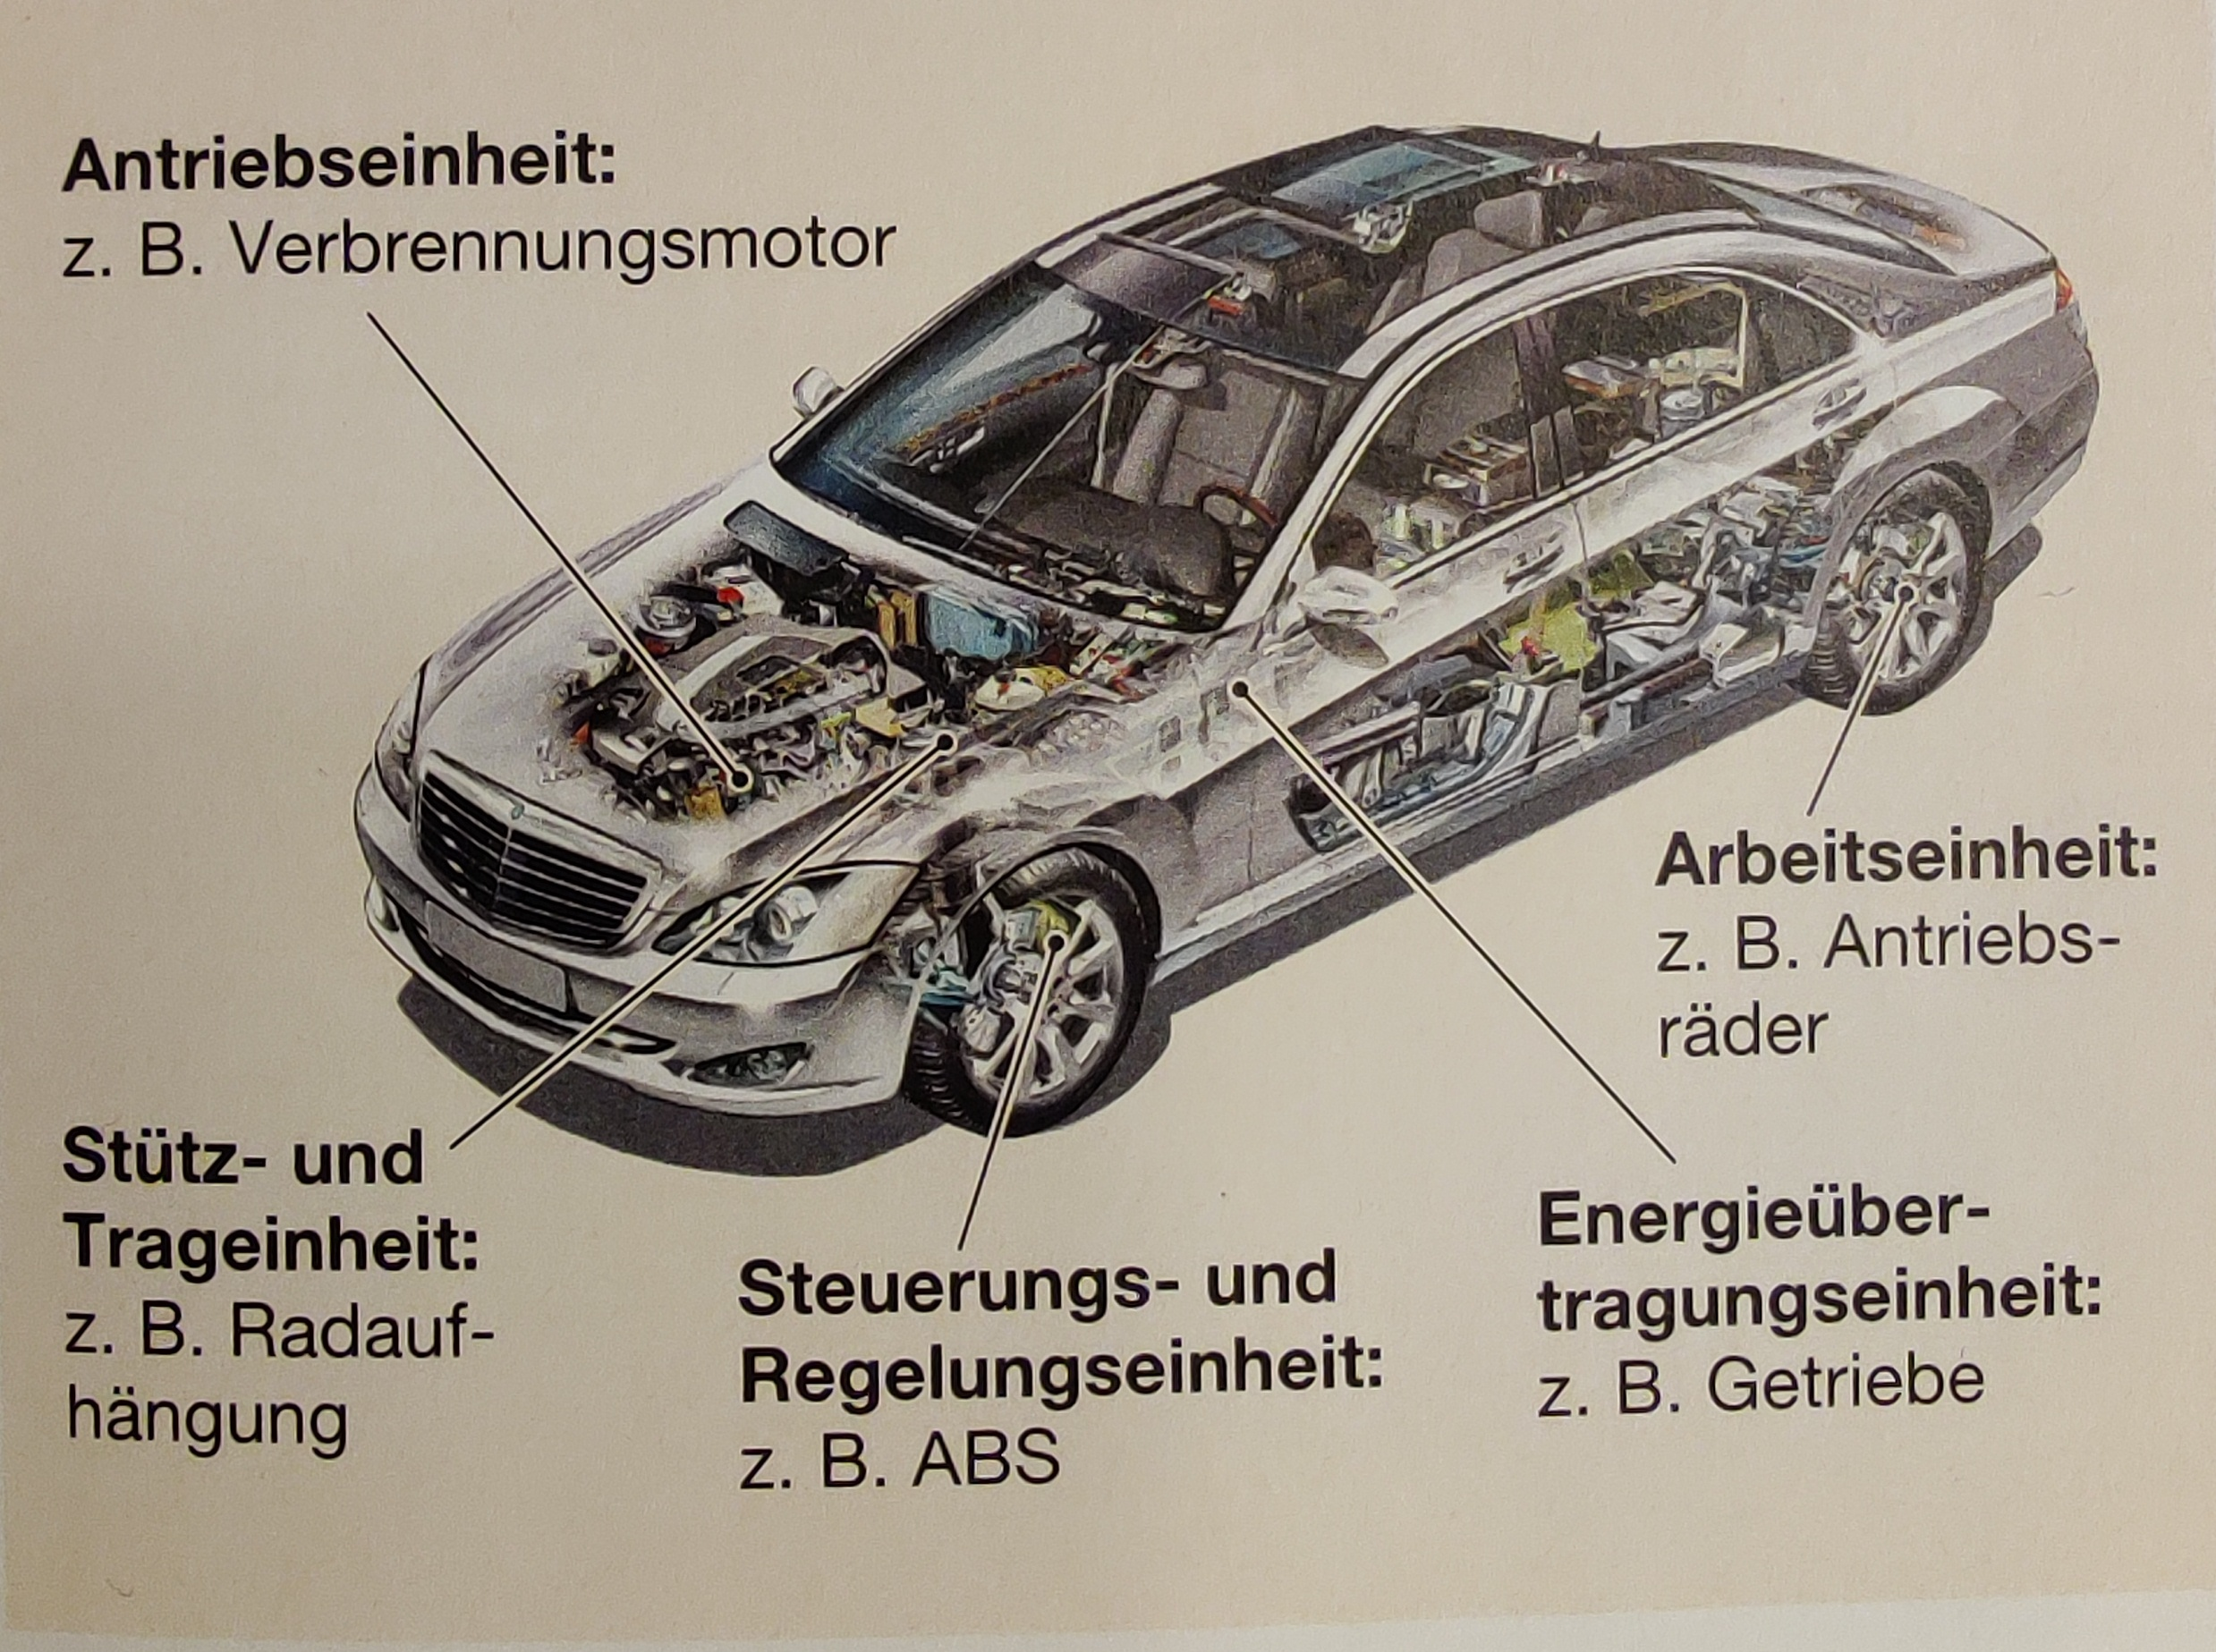
\includegraphics[scale=0.1]{assets/figures/Teilsysteme des Kraftfahrzeugs.jpg}
	\begin{flushleft}
		Quelle: Westermann S. 19
	\end{flushleft}
	\label{fig:birds}
\end{figure}


\subsubsection{Antriebseinheit}
Die Antriebseinheit wandelt die zugeführte Energie in die erforderliche Antriebsenergie um.
Diese Umwandlung wird im Motor durchgeführt.
Hauptsächlich werden Elektro- und Verbrennungsmotoren eingesetzt.

Verbrennungsmotoren unterscheiden sich von Elektromotoren durch ihre Energieerzeugung.
Die Energieerzeugung wird durch die Verbrennung von Kraftstoff erzeugt.
Dazu wird ein Kraftstoff-Luft-Gemisch in einem Brennraum mit Kolben zur Verbrennung verwendet.
Durch die Verbrennung steigt der Druck im Brennraum stark an und bewegt einen Kolben.

\subsubsection{Arbeitseinheit}
Die Arbeitseinheit ist die Verbindung zwischen den Antriebsrädern und der Fahrbahn.
Durch die Bewegung der Antriebsrädern wird das Kraftfahrzeug in Bewegung gesetzt.

\subsubsection{Energieübertragungseinheit}
Die Energieübertragungseinheit leitet die Energie in der geforderten Bewegungsart und Bewegungsgeschwindigkeit zu der Arbeitseinheit weiter.

Energieübertragungseinheiten sind Baugruppen einer Maschine, die zur Übertragung von Energie benötigt werden.
Beispiel hierfür sind Kabel die elektrische Energie leiten oder Wellen, Zahnräder und Riemen die mechanisches Drehmoment übertragen.

\subsubsection{Stütz- und Trageeinheit}
Der Rahmen oder der selbsttragende Aufbau eines Kraftfahrzeuges ist die Stütz- und Trageeinheit.
Diese haben hauptsächlich die Aufgabe, die Teilsysteme aufzunehmen und zu einer Einheit zu verbinden.

\subsubsection{Steuerungs- und Regelungseinheit}
Die Steuerungs- und Regelungseinheit beeinflusst die Stoff- und Energieumsetzung durch Informationsverarbeitung.

\subsubsection{Steuerungseinheit}
Bei der Steuerungseinheit werden verschiedene Eingangsgrößen durch das System in eine oder mehrere Ausgangsgrößen verändert.
Beispiele für Steuerungen sind:
\begin{itemize}
	\item Klimaanlage: Es wird eine Solltemperatur eingestellt.
	      Die Klimaanlage kühlt konstant.
	      Die Klimaanlage kühlt solange mit dieser eingestellten Temperatur solange sie nicht verändert wird.
	      Die Umgebungstemperatur wird nicht berücksichtigt.
	\item Licht: Der Schalter wird betätigt und das Licht wird eingeschaltet.
	      Das Licht bleibt permanent eingeschaltet.
	      Das Licht geht erst aus wenn der Schalter ausgeschaltet wird.
	      Das Umgebungslicht wird nicht berücksichtigt.
\end{itemize}

\newpage

\subsubsection{Regelungseinheit}
Bei einer Regelungseinheit werden die Eingangsgrößen mit einem Sollwert verglichen und so lange angepasst bis der Sollwert erreicht wird.
Beispiele für Regelungen sind:
\begin{itemize}
	\item Klimaautomatik: es wird eine Solltemperatur eingestellt.
	      Es wird gemessen wie warm oder wie Kalt die Temperatur ist.
	      Sollte die Temperatur unter der Solltemperatur liegen, wird die Klimaautomatik auf Heizen gestellt.
	      Sollte die Temperatur über der Solltemperatur liegen, wird die Klimaautomatik auf Kühlen gestellt.
	\item Lichtautomatik: Es gibt eine Schwelle bei der das Licht eingeschaltet werden soll.
	      Es gemessen wie hell das Umgebungslicht ist.
	      Sollte das Umgebungslicht zu gering sein wie zum Beispiel im Tunnel oder bei Dämmerung wird das Licht eingeschaltet.
	      Sobald das Umgebungslicht wieder hell genug ist zum Beispiel beim verlassen des Tunnels oder bei Sonnenaufgang, wird das Licht wieder ausgeschaltet.
\end{itemize}

\subsection{Fahrzeugklassen}

Kraftfahrzeuge können Bauartbedingt in Kategorien eingeordnet werden.
Die EU Kommission hat hierfür acht Klassen definiert.\footnote{VERORDNUNG (EU) Nr. 678/2011 DER KOMMISSION
	vom 14. Juli 2011, TEIL A ABS.1 - https://eur-lex.europa.eu/eli/reg/2011/678/oj?locale=de}

\begin{itemize}
	\item Klasse L: Leichte ein- und zweispurige Kraftfahrzeuge
	\item Klasse M: Vorwiegend für die Beförderung von Fahrgästen und deren Gepäck ausgelegte und gebaute Kraftfahrzeuge
	\item Klasse N: Vorwiegend für die Beförderung von Gütern ausgelegte und gebaute Kraftfahrzeuge
	\item Klasse O: Anhänger, die sowohl für die Beförderung von Gütern und Fahrgästen als auch für die Unterbringung von Personen ausgelegt und gebaut sind
	\item Klasse S: unvollständige Fahrzeuge, die der Unterklasse der Fahrzeuge mit besonderer Zweckbestimmung zugeordnet werden soll
	\item Klasse R: Anhänger, die in der Land- und Forstwirtschaft verwendet werden
	\item Klasse S: Maschinen, die in der Land- und Forstwirtschaft zum Einsatz kommen und gezogen werden
	\item Klasse T: Zugmaschinen, die in der Land- und Forstwirtschaft verwendet werden wie Traktoren
	\item Klasse C: Zugmaschinen, die in der Land- und Forstwirtschaft verwendet werden und auf Ketten laufen wie ein Bagger
\end{itemize}

Die relevantesten Klassen sind M und N.
\vspace{0.5cm}

\subsection{Klasse M}
In der Klasse M werden Kraftfahrerzeuge eingeordnet die für die Beförderung von Personen und Gepäck zuständig sind und mindestens 4 Räder haben sowie eine Hochgeschwindigkeit von über 25 \ac{kmh} haben.
\newline
Die Klasse M spaltet sich in 3 Unterklassen auf:
\begin{itemize}
	\item {Klasse M1}
	\item {Klasse M2}
	\item {Klasse M3}
\end{itemize}
\subsubsection{Klasse M1}
Kraftfahrzeuge der Klasse M1 haben über die Eigenschaften der Klasse M noch folgende weitere Eigenschaften:
\begin{itemize}
	\item {nicht mehr als 8 Sitzplätze und 1 Platz für den Fahrer}
	\item {keine Stehplätze}
	\item {zulässiges Gesamtgewicht von maximal 3,5 \ac{t}}
\end{itemize}

In der Klasse M1 sind Kraftfahrzeuge wie Personenkraftwagen(Limousine, Cabrio) und Wohnmobile zu finden.

\subsubsection{Klasse M2}
Kraftfahrzeuge der Klasse M2 haben über die Eigenschaften der Klasse M noch folgende weitere Eigenschaften:
\begin{itemize}
	\item {mehr als 8 Sitzplätze}
	\item {zulässiges Gesamtgewicht von maximal 5 \ac{t}}
\end{itemize}

In der Klasse M2 sind Kraftfahrzeuge wie ein Eindecker-Bus bis 5 \ac{t} oder ein Doppeldecker-Bus bis 5 \ac{t} zu finden.

\subsubsection{Klasse M3}

Die dritte Unterklasse der Klasse M ist M3.

Kraftfahrzeuge der Klasse M3 haben über die Eigenschaften der Klasse M noch folgende weitere Eigenschaften:
\begin{itemize}
	\item {mehr als 8 Sitzplätze}
	\item {zulässiges Gesamtgewicht von über 5 \ac{t}}
\end{itemize}

In der Klasse M3 sind Kraftfahrzeuge wie ein Eindecker-Bus über 5 \ac{t} oder Doppeldecker-Bus über 5 \ac{t} zu finden.

\subsection{Klasse N}
In der Klasse N werden Kraftfahrerzeuge eingeordnet die für die Beförderung von Gütern zuständig sind und mindestens 3 Räder haben sowie ein zulässiges Gesamtgewicht von über 1 \ac{t} haben.
Die Klasse N spaltet sich in 3 Unterklassen auf:
\begin{itemize}
	\item {Klasse N1}
	\item {Klasse N2}
	\item {Klasse N3}
\end{itemize}

\subsubsection{Klasse N1}
Fahrzeuge zur Güterbeförderung mit einer zulässigen Gesamtmasse bis zu 3,5 \ac{t}.
In der Klasse N1 sind Kraftfahrzeuge die in dicht besiedelten Regionen gut zurecht kommen, wie Paketzusteller oder Fahrzeuge der Post.


\subsubsection{Klasse N2}
Fahrzeuge zur Güterbeförderung mit einer zulässigen Gesamtmasse von zu 3,5 \ac{t} bis 12 \ac*{t}.
In der Klasse N2 sind Kraftfahrzeuge die regional Güterbefördern, dies könnten Kraftfahrzeuge die Waren aus einem Zentrallager in die Filialen transportieren.
Diese Kraftfahrzeuge sind darauf ausgelegt hunderte Kilometer zurückzulegen.


\subsubsection{KLasse N3}
Fahrzeuge zur Güterbeförderung mit einer zulässigen Gesamtmasse von mehr als 12 \ac{t}.
In der Klasse N3 sind Kraftfahrzeuge die überregional Güterbefördern, wie ein Kraftfahrzeug das große Mengen an Ladung fassen kann und darauf ausgelegt sind tausende Kilometer zurückzulegen.

\subsection{Autonome Kraftfahrzeuge}
Beim autonomen Fahren, fährt ein Kraftfahrzeug verwaltungsgemäß selbständig.
Für Kraftfahrzeuge wurden von der \ac{SAE} Automatisierungsstufen definiert\cite{PRACTICE}.
\begin{itemize}
	\item Stufe 0 (Keine Automation)
	\item Stufe 1 (Assistenzsysteme)
	\item Stufe 2 (Teilautomatisierung)
	\item Stufe 3 (Bedingte Automatisierung)
	\item Stufe 4 (Hochautomatisierung)
	\item Stufe 5 (Vollautomatisierung)
\end{itemize}
\subsubsection{Was passiert in den Stufen?}
Die Stufen unterscheiden sich im wesentlichen nur durch die Anzahl der Automatisierungsgrade.

\vspace{0.5cm}

In der Stufe 0 (Keine Automation):
\begin{itemize}
	\item keine Assistenzsysteme
	\item Kraftfahrzeug kann keine Fahraufgaben übernehmen
	\item Fahrer kontrolliert permanent das Fahrzeug
\end{itemize}

\vspace{0.5cm}

In der Stufe 1 (Assistenzsysteme):
\begin{itemize}
	\item Assistenzsysteme wie zum Beispiel ein System zur automatischen Geschwindigkeitsregelung oder eine Berganfahrhilfe
	\item Fahrer hat eine passive Unterstützung bei Fahraufgaben
	\item Kraftfahrzeug kann keine Fahraufgaben übernehmen
	\item Fahrer kontrolliert permanent das Fahrzeug
\end{itemize}

\vspace{0.5cm}

In der Stufe 2 (Teilautomatisierung):
\begin{itemize}
	\item Assistenzsysteme, wie zum Beispiel der Spurführungsassistent oder Stauassistent
	      \begin{itemize}
		      \item automatisch bremsen
		      \item automatisch beschleunigen
		      \item automatisch lenken
	      \end{itemize}
	\item Kraftfahrzeug kann Fahraufgaben teilautomatisiert übernehmen
	\item Fahrer kann sich für kurze Zeit von den Fahraufgaben abwenden
	\item Fahrer muss jeder Zeit die teilautomatisierte Fahraufgabe übernehmen können
\end{itemize}

\vspace{0.5cm}

In der Stufe 3 (Bedingte Automatisierung):
\begin{itemize}
	\item hochautomatisierte Assistenzsysteme
	\item Kraftfahrzeug kann Fahraufgaben unter bestimmten Voraussetzungen vollständig übernehmen
	\item Fahrer kann sich unter bestimmten Voraussetzungen von den Fahraufgaben abwenden
	\item Fahrer muss innerhalb von wenigen Sekunden die Fahraufgabe übernehmen können
\end{itemize}

\vspace{0.5cm}

In der Stufe 4 (Hochautomatisierung):
\begin{itemize}
	\item hochautomatisierte Assistenzsysteme
	\item Kraftfahrzeug kann Fahraufgaben in hochkomplexen Verkehrssituationen vollständig übernehmen
	\item Fahrer kann sich von den Fahraufgaben abwenden
	\item Fahrer muss fahrtüchtig sein, um im Bedarfsfall die Fahraufgabe übernehmen zu können
\end{itemize}

\vspace{0.5cm}

In der Stufe 5 (Vollautomatisierung):
\begin{itemize}
	\item hochautomatisierte Assistenzsysteme
	\item Kraftfahrzeug übernimmt alle Fahraufgaben vollständig
	\item Fahrer ist nicht erforderlich
	\item alle Personen im Wagen werden zu Passagieren
\end{itemize}


Autonome Kraftfahrzeuge sind Kraftfahrzeuge die nicht nur automatisch fahren sondern von einem System gesteuert werden.
Somit sind diese Kraftfahrzeuge aus Sicht der Nutzenden autonom.

Während manche in der Verbreitung autonomer Kraftfahrzeuge die Lösung vieler Probleme sehen können,
vermuten andere eine Verschlechterung der Verkehrs- und Umweltlage.

Die Bedeutung von autonomen Kraftfahrzeugen hängt sowohl von der technischen Komplexität als auch von den politischen Regulierung ab.

In welchem Maß das Level 5 System im Straßenverkehr teilnimmt entscheidet vorerst der gesetzliche Rahmen.
Dies ist wiederum abhängig wie der zukünftige Verkehr aussehen soll.
\subsection{Umweltbelastungen durch Kraftfahrzeuge}
Kraftfahrzeuge belasten die Umwelt auf verschiedene Arten.
Hierunter fallen
die Erzeugung von Rohstoffen für Materialien die für die Produktion von Kraftfahrzeugen benötigt werden,
die tatsächliche Produktion von Kraftfahrzeugen,
der Betrieb von Kraftfahrzeugen,
sowie die Entsorgung von Kraftfahrzeugen.

Gerade der Betrieb von Kraftfahrzeugen belastet die Umwelt durch die verschieden Arten von Schadstoffen.
Unterschieden wird die Art der Belastung,
durch die Verbrennung entstandene Abgase,
Feinstaub der durch die Verbrennung, sowohl auch durch den Abrieb von Reifen und Bremsen freigesetzt wird
und die Infrastruktur der Straßen, Parkplätze und anderer Einrichtungen.

\subsection{Verbrennungsabgase}
Durch Verbrennung von Kraftstoffen entstehen verschied giftige Schadstoffe:
\begin{itemize}
	\item {\ac{CO}}
	\item {\ac{NO}}
	\item unverbrannte Kohlenwasserstoffe (HC)
\end{itemize}
Die Abgase strömen nach der Verbrennung im Verbrennungsraum durch die Abgasanlage in die Umwelt.
Es gibt auch ungiftige Stoffe die durch die Verbrennung abgegeben werden wie \ac{zb} \ac{Wasser} und \ac{CO2}.
Die Menge der Abgase die durch die Abgasanlage strömen ist von der Größe des Motors sowie dem Lastzustand des Motors abhängig.

\subsection{Feinstaub}
Feinstaub ist ein fester oder flüssiger Stoff der nicht sofort zu Boden sinkt.
Neben der Art des Feinstaubes ist unter anderem die Wetterlage für die Verbreitung und Absenkung von Feinstaub entscheidend.

Luftfeuchtigkeit beeinträchtigt die Ausbreitung von Feinstaub da sich dieser bei geringer Luftfeuchtigkeit länger in Luft halten kann sich besser ausbreiten kann.

Feinstäube werden als Particle Matter (PM, zu deutsch Stoffteilchen) bezeichnet. Diese Luftschadstoffe sind gesundheitsschädlich.

Unterschieden wird zwischen Feinstaub der aus natürlichen Quellen entstanden ist und Feinstaub der durch menschliches Handeln entstanden ist.

\subsubsection{Feinstaub aus natürlichen Quellen}
Natürlicher Feinstaub entsteht ohne menschliches Handeln durch:
\begin{itemize}
	\item Vulkane
	\item Wald- und Buschbrände
	\item Pollen
	\item Sporen
\end{itemize}


\subsubsection{Feinstaub durch menschliches Handeln}
Feinstaub der durch menschliches Handeln entstanden ist wird auch anthropogener Feinstaub genannt.
Feinstaub durch menschliches Handeln entsteht durch:
\begin{itemize}
	\item Verbrennung und Abrieb vom Straßenverkehr
	\item Verbrennungsabgase von Kraftwerken und Müllverbrennungsanlagen
	\item Brände von Gegenständen
	\item Industrieprozesse wie die Stahlerzeugung
\end{itemize}

Einrichtungen der Umweltzonen und Festlegung von Fahrverboten durch die Kommunen und Städte können zur Verbesserung der Luftreinhaltung führen.
Das befahren einer Umweltzone ist dann nur mit einer entsprechenden Kennzeichnung des Fahrzeuges möglich, die man bei der zuständigen Behörde erlangen kann.



\subsection{Infrastruktur}
Auch die Infrastruktur belastet die Umwelt, indem:
\begin{itemize}
	\item Wälder abgeholzt werden um die Verkehrsanbindung zu verbessern
	\item Straßen vergrößert um ein höheres Verkehrsaufkommen zu bewältigen
	\item starke Erhitzung durch Sonneneinstrahlung auf dunklen Verkehrswegen
	\item Grünflächen abgeschafft werden um mehr Parkmöglichkeiten zu gewinnen
\end{itemize}


\section{Umweltbelastung nach Bedingungen}
Die Umweltbelastung kann stark nach Betriebszuständen variieren.
So verbraucht ein Fahrzeuge das bergab fährt weniger Kraftstoff und stößt somit auch weniger Luftschadstoffe aus.
Die Umweltbelastung durch Luftschadstoffe hängt von folgendem ab:
\begin{itemize}
	\item dem Fahrverhalten des Fahrers, wie dem Beschleunigungsverhalten und der Fahrgeschwindigkeit ab
	\item der Effizienz des Fahrzeugs, je effizienter desto besser
	\item dem Gewicht des Fahrzeugs, je leichter desto weniger Gewicht muss beschleunigt und gebremst werden
	\item der Fahrstrecke, fährt das Fahrzeug eine Steigung wird mehr Kraftstoff benötigt
	\item dem Wetter, je nach Wind wird mehr oder weniger Kraftstoff benötigt
	\item dem Betriebszustand, wenn sich das Fahrzeug nicht im Betriebszustand befindet wird Energie verwendet um den Betriebszustand zu erreichen
\end{itemize}







\section{Assistenzsysteme}
\subsection{Keine Assistenzsysteme}
\subsection{Assistenzsysteme}
\subsection{Teilautomatisierung}
\subsection{Bedingte Automatisierung}
\subsection{Hochautomatisierung}
\subsection{Vollautomatisierung}

\chapter{Problemlösung durch Assistenzsysteme}
\section{}


% !!! hier kann man Beispiele aufführen, wie zb Bus, PKW, LKW; Traktor
% !!! Wie groß ist der Anteil der Kraftfahrzeuge in den Klassen in Deutschland?
% !!! Warum und wie blesatst jede Klasse die Umwelt?
% !!! PKW durch unnötige Kurzstecke
% !!! Sinnloses laufenlassen von LKW
% !!! Zustellungen von Gütern
% !!! Leerfahrten


% \subsection{Autonomes Fahren}

% !!! Was sind autonome fahrzeuge?
% !!! Welche 


% Beim autonomen Fahren, fährt ein \ac{Kfz} Verwaltungsgefäß selbständig.
% Für \ac{Kfz} wurden von der \ac{SAE} Institut in der Norm SAE J3016\footnote{SAE J3016\textunderscore202104 - https://www.sae.org/standards/content/j3016\textunderscore202104} Automatisierungsgrade definiert.
% \begin{itemize}
% 	\item Stufe 0 (Keine Automation)
% 	\item Stufe 1 (Assistenzsysteme)
% 	\item Stufe 2 (Teilautomatisierung)
% 	\item Stufe 3 (Bedingte Automatisierung)
% 	\item Stufe 4 (Hochautomatisierung)
% 	\item Stufe 5 (Vollautomatisierung)
% \end{itemize}
% \subsubsection{Was passiert in den Stufen?}
% Die Stufen unterscheiden sich im wesentlichen nur durch die Anzahl der Automatisierungsgrade.

% \vspace{0.5cm}

% In der Stufe 0 (Keine Automation):
% \begin{itemize}
% 	\item keine Assistenzsysteme
% 	\item \ac{Kfz} kann keine Fahraufgaben übernehmen
% 	\item Fahrer ist unter permanenter Kontrolle
% \end{itemize}

% \vspace{0.5cm}

% In der Stufe 1 (Assistenzsysteme):
% \begin{itemize}
% 	\item Assistenzsysteme wie \ac{GRA} oder eine Berganfahrhilfe
% 	\item Fahrer hat eine passive Unterstützung bei Fahraufgaben
% 	\item \ac{Kfz} kann keine Fahraufgaben übernehmen
% 	\item das \ac{Kfz} ist unter permanenter Kontrolle des Fahrers
% \end{itemize}

% \vspace{0.5cm}

% In der Stufe 2 (Teilautomatisierung):
% \begin{itemize}
% 	\item Assistenzsysteme, wie der Spurführungsassistent oder Stauassistent
% 	      \begin{itemize}
% 		      \item automatisch bremsen
% 		      \item automatisch beschleunigen
% 		      \item automatisch lenken
% 	      \end{itemize}
% 	\item \ac{Kfz} kann Fahraufgaben teilautomatisiert übernehmen
% 	\item Fahrer kann sich für kurze Zeit von den Fahraufgaben abwenden
% 	\item Fahrer muss jeder Zeit die Fahraufgabe übernehmen können
% \end{itemize}

% \vspace{0.5cm}

% In der Stufe 3 (Bedingte Automatisierung):
% \begin{itemize}
% 	\item hochautomatisierte Assistenzsysteme
% 	\item \ac{Kfz} kann Fahraufgaben unter bestimmten Voraussetzungen vollständig übernehmen
% 	\item Fahrer kann sich unter bestimmten Voraussetzungen dauerhaft von den Fahraufgaben abwenden
% 	\item Fahrer muss innerhalb wenigen Sekunden die Fahraufgabe übernehmen können
% \end{itemize}

% \vspace{0.5cm}

% In der Stufe 4 (Hochautomatisierung):
% \begin{itemize}
% 	\item hochautomatisierte Assistenzsysteme
% 	\item \ac{Kfz} kann Fahraufgaben in hochkomplexen Verkehrssituationen vollständig übernehmen
% 	\item Fahrer dauerhaft von den Fahraufgaben abwenden
% 	\item Fahrer muss fahrtüchtig sein, um im Bedarfsfall die Fahraufgabe übernehmen zu können
% \end{itemize}

% \vspace{0.5cm}

% In der Stufe 5 (Vollautomatisierung):
% \begin{itemize}
% 	\item hochautomatisierte Assistenzsysteme
% 	\item \ac{Kfz} übernimmt alle Fahraufgaben vollständig
% 	\item Fahrer ist nicht erforderlich
% 	\item alle Personen im Wagen werden zu Passagieren
% \end{itemize}



